\newcommand{\op}{\operatorname}
\newcommand{\ind}{\stackrel{ind.}{\sim}}
\section{Introduction}
The statistical problem of comparing group in gene expression studies is an example of the $n \ll p$ paradigm. Recently, RNA-seq technology has supplanted microarrays as the primary platform for these studies. As the technology has developed, statistical methods to analyze the data these technologies produce has proliferated. A common element of such methods is the regularization of gene-specific analysis to decrease false detection rates and improve model accuracy. One way to acheive this is to employ appropriate hierarchical models. In this paper we present a nonparametric Bayesian hierarchical regression model, applicable to a large class of gene expression studies.
%Because the presence of a meaningful biological effect fits awkwardly into the framework, we approach the problem of  addressed through estimation \citet{deseq2014}. This is the approach that we pursue here.

% Current estimation methodologies can be understood as improving upon a ``straight" estimator by modeling gene-specific model parameters to borrow information across genes. \textit{Insert analogy to Stein's estimator}.

Because the data is expensive to collect, gene expression studies typically have fairly small sample sizes ($N \approx 10$). However, because there are many genes to observe, a gene expression experiment presents an opportunity to learn the underlying distribution of the gene-specific parameters, $\mathcal{P}$. Given that gene profiling studies typically measure expression of tens of thousands of genes, there is substantial information to estimate $\mathcal{P}$. If we assume a standard parameteric family form for $\mathcal{P}$, then we should be able to estimate $\mathcal{P}$ precisely. We use the term ``hierarchical model" to refer to models where some or all of the parameters involved in the data generation model are themselves modeled as random variables.
% The advantages of such hierarchical models have been shown to work well in practice, regardless of whether the distributional form of the random effects restrict should be assumed to have a simple form, will tend to be estimated very precisely. If the model is overly simplistic, the information borrowed across genes will tend to be quite vague. 
A rationale for hierarchical modeling in gene expression is to regularize estimation for gene-specific parameters by shrinking the posterior distribution of these parameters toward the mass of their distribution. Largely for computational reasons, empirical Bayes methods have been preferred to fully Bayesian methods. One argument for their use is that when $G$ is large, $\mathcal{P}$ should be have low variance in the posterior, so that inference based on an estimate of $\mathcal{P}$ should be quite similar to a fully Bayesian analysis which integrates over the uncertainty in $\mathcal{P}$. The findings of Landau (2016) support this claim.

Whether the method used is empirical Bayes or fully Bayesian, the use of hierarchical models in this area has led to critical improvements in estimation and testing. \citet{niemi} observed that the choice of parametric family can impact both estimation and the ranking of genes. It seems that appropriate modeling of the underlying distribution of the gene-specific parameters will lead to better results; in contrast, misspecification of the distribution will limit both the accuracy and precision that can be obtained in estimation of the parameters.
%The theory which supports these arguments assumes that the complexity of $\mathcal{P}$ can be described by a fixed number of parameters.
%Whether or not a suitable, parsimonious parameteric model can be found for the gene-specific parameters in gene expression data is a question that 
% Indeed, many `shrinkage priors', or equivalent methods, has proven to be a useful tool even when the distributional form is misspecified.

% Because of its essential role, the shape of the tail, vis a vis the choice of the hierarchical model, should be considered. We showed that the choice affected the number of genes called as well as which ones.

Several interesting approaches to improving the hierarchical model have been considered. \citet*{lithio} considered reparameterizing the linear predictors to minimize the correlations of the gene-specific effects, in part to motivate the use of independent prior distributions. They find that the parameterization has a significant impact on the performance of the model. 
%We hope avoid such sensitivities by using nonparametric prior distributions for these parameters.
\citet{voom} proposed a method which unlocks linear modeling of RNA-seq data by estimating precision weights for each RNA-seq count. This is accomplished by estimating the mean variance relationship parametrically by fitting a loess curve using independent estimates by gene of the average log expression and fourth root of the error variance. This between-gene information is then applied within genes via precision weights. \citet{liu} proposed a semiparametric model for differential expression. In their model, a gamma mixture of Poisson was used and information was borrowed across genes only for the log-fold-change parameter, which was given a Dirichlet process prior.

In the present article, we propose a Bayesian nonparametric model which extends the approach taken in \citet{liu} by modeling the joint distribution of all gene-specific parameters with a Dirichlet process. We assume a normal data model, using voom weights to accomodate the mean-variance relationship of RNA-seq count data. The goal of this work is to provide a method that flexibly models the gene-specific parameters, learning their distribution automatically. For computation of the posterior, we exploit conditional independence within the posterior distribution to parallelize the computation on GPUs, following the outline presented in \citet{suchard}.
% \citet{landau-compute} implemented a Gibbs sampler for a parametric Bayesian hierarchical model for RNA-seq data using a graphics processing unit (GPU) to accelerate computation. Their work helped to inspired this Bayesian nonparametric approach. 


\section{RNA-seq gene expression data}
\label{sec:data}
The starting point for our analyses is an array of RNA-seq total aligned read counts measuring the abundance of a particular messenger RNA transcript in a sample. Such an array consists of $G$ rows and $N$ columns, corresponding to genes and samples, respectively. The abundance of a transcript is often referred to as gene expression; we will follow this convention here. For more details on data collection and preprocessing of RNA-seq data, please see Nettleton and Datta (2016).

A simple analysis of RNA-seq data may be acheived by analyzing each gene independently. The experimental design can generally considered the same for all genes. Select rows for an example data set are shown below in Table \ref{tab:ex-1}.

\begin{table}[ht]
\centering
\begin{minipage}{.8\textwidth}
\caption{\small Sample of RNA-seq total read counts from \citep{paschold}. Columns names identify samples, including the genotype and a replicate number, from which we can infer the flow cell that was used for sequencing. Gene annotation information (regarding the rows), is not used for in our analysis. The first and last genes listed strongly indicate differential expression between the two inbred maize lines.}
\end{minipage}
\label{tab:ex-1}
\vspace{.25cm}
\begin{tabular}{lrrrrrrrr}
  \hline
& $\mbox{B73}_1$ & $\mbox{B73}_2$ & $\mbox{B73}_3$ & $\mbox{B73}_4$ & $\mbox{Mo17}_1$ & $\mbox{Mo17}_2$ & $\mbox{Mo17}_3$ & $\mbox{Mo17}_4$ \\ 
  \hline
$\mbox{gene}_1$ & 666 & 590 & 654 & 703 &   3 &   3 &   1 &   1 \\ 
$\mbox{gene}_2$& 414 & 422 & 383 & 416 & 392 & 346 & 402 & 351 \\ 
  $\mbox{gene}_3$ & 1525 & 1530 & 904 & 833 & 1688 & 1568 & 1413 & 1377 \\ 
  $\mbox{gene}_4$ &  12 &  11 &   5 &   2 &   8 &  20 &   9 &   6 \\ 
  $\mbox{gene}_5$ &   1 &   1 &   0 &   2 & 951 & 945 & 1157 & 867 \\ 
   \hline
\end{tabular}
\end{table}

\subsection{Maize data of Paschold et al.}
THIS IS PLAGARISM AT THIS POINT:
We use as a motivating example a maize data set \citep{paschold} of RNA-seq gene expression in parental lines B73 and Mo17 and the reciprocal hybrid genotypes (B73$\times$Mo17, Mo17$\times$B73) with a total of 39,656 genes. Each variety had four biological replicates measured with Illumina methodology and equipment. Reads were mapped to the whole reference genome using the short reads aligner, NOVOALIGN. For more specifics, please see \cite{paschold}.

Heterosis exists when the expected value of a hybrid phenotype differs from the average of the expected phenotypic values of the hybrid's parents.  The most interesting and useful form of heterosis, known as hybrid vigor, occurs when hybrid progeny display a mean phenotype that is superior to  both parental phenotypic means.  This heterosis phenomenon was scientifically documented in plants by \cite{darwin1876effects} and has long been used to improve agricultural production. One classic example involves hybrid maize offspring that are taller, faster to mature, and yield considerably more grain than their inbred parents \citep{hallauer1981quantitative, hallauer2010quantitative}.

There is interest in using gene expression data to help identify genes that drive heterosis; i.e. where the mean gene expression of the hybrid is high relative to its parents.

\subsection{Normalization and weighting}
\paragraph{Normalization}
Artifacts of the sequencing procedure can lead to some samples having larger or smaller read counts on average relative to other sample. This introduces biases that require adjustment. These corrections are typically made at the time of analysis by introducing a sample specific offset. Different methods for normalization have been proposed. \citet{robinson2010} proposed a method called trimmed mean of M-values (TMM) to correct between-sample biases by compare observed log-fold-change values between samples for all genes. Under the assumption that most genes are not differentially expressed, they use a trimmed mean to robustly estimate the bias. When there are more than two samples, the same methodology is extended by using one sample as a reference. For details, see \citet{robinson2010}.

\paragraph{Precision weights adjust for non-contant variance}
Theory suggests that an RNA-seq count, $C$, would have a Poisson distribution, with variance equal to the mean ($\op{V}(C|\mu)=\mu, \mu=\op{E}(C)$), if the RNA from the same sample were sequenced repeatedly. Biological variation (either between subjects or through repeated sampling) leads overdispersion of the counts. Often, the negative binomial distribution is used because its variance is quadratic with the mean ($\op{V}(C|\mu)=\mu+\phi\mu^2$). Because gene expression is usually measured on the log scale, through an application of the delta method, we can re-express this approximately in terms of the log-count ($\op{V}(\log C|\mu) \approx \frac{1}{\mu} + \phi$. While this assumption may be adequate for genes with similar expression levels, empirical studies suggest that the overdispersion parameter, $\phi$, tends to be larger for genes with lower expression than those with higher expression.

\cite{voom} proposed \textit{voom}, a way to incorporate between-gene information about the mean-variance relationship in an RNA-seq data set through precision weighting of individual log-counts, making the data amenable to analysis with a linear model. It works by first calculating, for each gene, a sample standard deviation and mean log-count, and then fitting a LOWESS curve, treating the square root standard deviation as a response and the mean log-count as the predictor. Fitted values are then calculated for all counts, which are converted into precision weights.

Rather than assuming the mean-variance relationship of the negative binomial and allowing for an adjustment of the degree of overdispersion from gene to gene, voom's precision weighting scheme estimates the mean-variance relationship from the data and assumes that it applies both within as well as across genes. We use the precision weights as an input to our model (Section \ref{sec:model}) which estimates a gene-specific variance parameter. Our use of voom in our pipeline implies a gene-specific mean-variance relationship \textit{for the log counts} given by
$$\op{V}(\log C|\mu)=\sigma^2_g \widehat{\op{V}_{voom}(\log C|\mu)}.$$



\section{Bayesian nonparametric model}
The advantage of hierarchical modeling generally is that that by assumming a distribution, $\mathcal{P}$, on some parameters $\theta_g$ and by allowing the parameters of $\mathcal{P}$ to be learned from the data, we can borrow information across groups to reduce our uncertainty about $\theta_g$. An implication of the misspecification of the distribution on the parameters can be that the utility of the hierarchical model is reduced; the information that the model is capable of borrowing is diminished.

\subsection{Illustration}
\label{subsec:illustration}
When the model assumptions on $\mathcal{P}$ restrict the posterior for $\mathcal{P}$ to a set that cannot realistically represent $\mathcal{P}$, this limits the efficiency of the hierarchical model. To illustrate, suppose we observe $y_{gn},\; g=1,\ldots,200,\;n=1,2,3$, and we are interested in hypotheses concerning $\op{E}(y_{gn})=\mu_g$. Suppose further that we can reasonably assume that $y_{gn}|\mu_g \ind \op{N}(\mu_g,\sigma^2)$, i.e. the data are conditionally normal, with a constant error variance. In this example we let $\mu_g$ be independent draws from a trivariate mixture of normals, $\mu_g \sim 1/3\op{N}(-4,1)+1/3\op{N}(0,1)+1/3\op{N}(4,1)$. This model was used to simulate a set of observations letting $\sigma^2=2$. A histogram of the the sample means, $\hat{\mu}_g$ is shown in the top panel of Figure~\ref{predictive}. Next, we fitted three Bayesian models to the data. First, $\mu_g \ind \mathcal{P}=\op{N}(\eta, \tau^2)$, with weakly informative priors on $\eta$ and $\tau^2$. Second, a mixture model with the correct number of components, $\mu_g \sim \mathcal{P}=\pi_1\op{N}(\eta_1,\tau^2)+\pi_2\op{N}(\eta_2,\tau^2)+\pi_3\op{N}(\eta_3,\tau^2)$, also with weakly informative priors on $\eta_j$ and $\tau^2$ and a $\op{Dir}(1,1,1)$ prior on $\pi$. Lastly, a Bayesian nonparametric prior: $\mu_g \ind \mathcal{P}$ with $\mathcal{P} \sim \op{DP}\left\{\alpha \op{N}(0,5^2)\right\}$. Critically, this last model allows us to be agnostic about the modality of $\mathcal{P}$; further details are given in the next section.

\begin{figure}[h!]
\centering
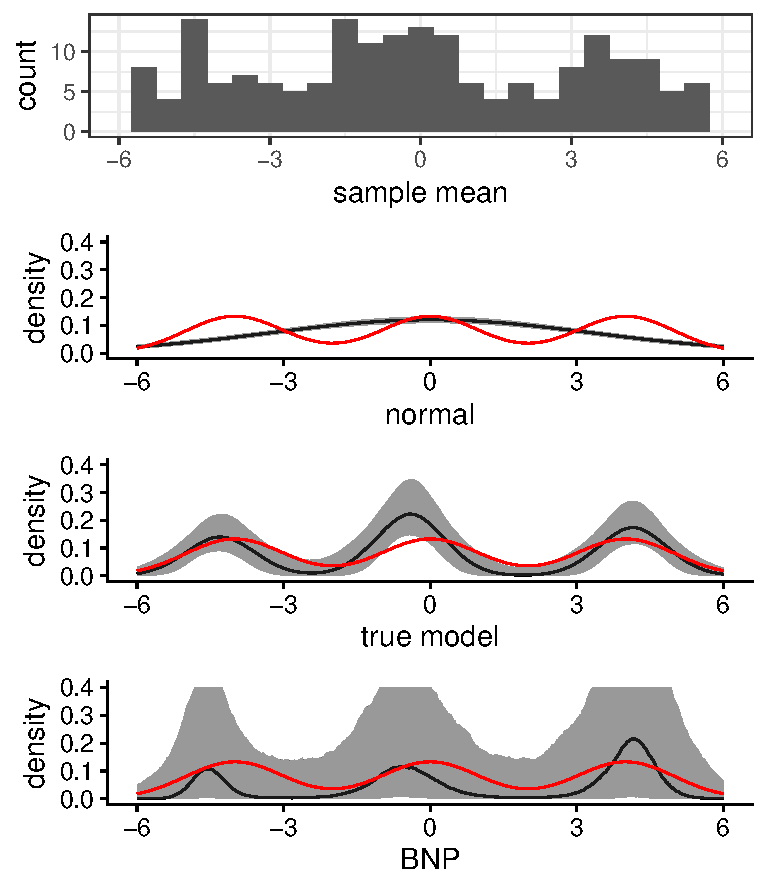
\includegraphics[width=.5\textwidth]{toy_ex/predictive}
\begin{minipage}{.7\textwidth}\small%
\caption{Top: Sample averages for simulated data of Section~\ref{subsec:illustration}. The next three rows correspond to pointwise posterior estimates and 90\% credible intervals for the underlying density corresponding to the random distribution, $\mathcal{P}$. For the BNP model, a weighted kernel density estimate employing a bandwidth of 0.1  was used for each posterior draws of $\mathcal{P}$, as the posterior draws do not have a density with respect to Lebesgue measure.}
\end{minipage}
\label{predictive}
\end{figure}


The bottom three panels of Figure \ref{predictive} show density estimates and 90\% pointwise credible intervals based on posterior samples of $\mathcal{P}|y$ for the three models. For the normal model and the ``true" model, these were computed by taking quantiles of the sampled density evaluated on a grid. For the Bayesian nonparameteric model, the sample density was estimated using a weighted kernel with bandwidth of 0.1 because samples of $\mathcal{P}$ do not have a density with respect to Lebesgue measure. The true generating model for the $\mu_g$ is shown in red. The posterior for the density of $\mu_g$ under the normal model has less uncertainty but is concentrated around an incorrect answer because of its inflexibility. Both the "true" and the BNP models contain much of the true density within the pointwise uncertainty intervals. The BNP model shows a great deal more posterior uncertainty because it does not assume a parametric model for $\mu_g$. Despite the increased uncertainty about $\mathcal{P}$, posterior estimation under the BNP model is nearly as good as under the true model; the left panel of Figure~\ref{precision} shows the lengths of the posterior 95\% credible intervals for the $\mu_g$ sorted by their length for the three models; the dotted lines represent correspond to a non-hierarchical analysis (indepedent, uniform priors on $\mu_g$) with $\sigma^2$ known ($+/- 4/\sqrt{3}$). For this data set, we see that both the nonparametric and true models have less posterior uncertainty than the normal model on average, while all three hierarchical models have substantially less uncertainty than a non-hierarchical model. The right panel shows histograms of the mean squared error, $\int (\mu_g - \mu_{g0})^2 p(\mu_g|y) d\mu_g$, computed for each $g$ under the three models, where $\mu_{g0}$ is the true value. Again, we see that estimation is substantially improved when $\mathcal{P}$ is modelled appropriately.

% \begin{figure}[h!]
% 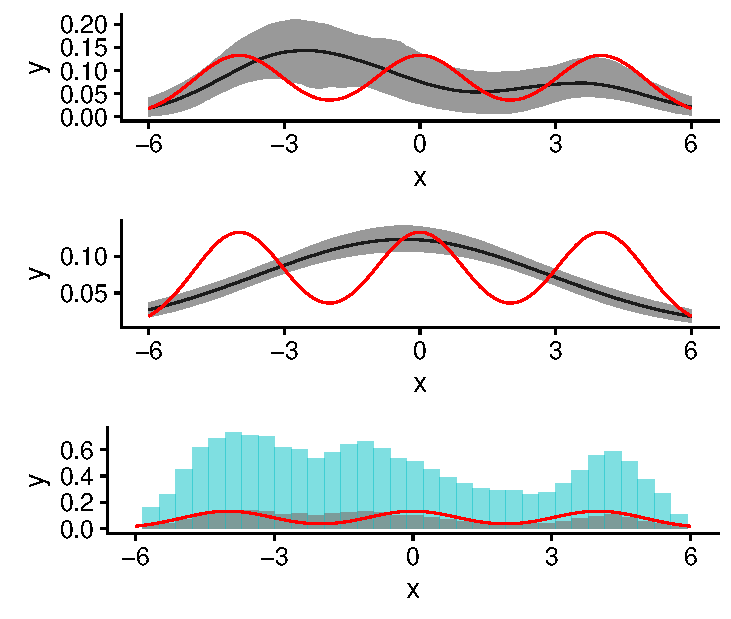
\includegraphics[width=.5\textwidth]{toy_ex/post-pred}
% \caption{Pointwise density estimates for three posterior models based on simulated data of Subsection~\ref{subsec:illustration}}
% \label{ex-predictive}
% \end{figure}

\begin{figure}[h!]
\centering
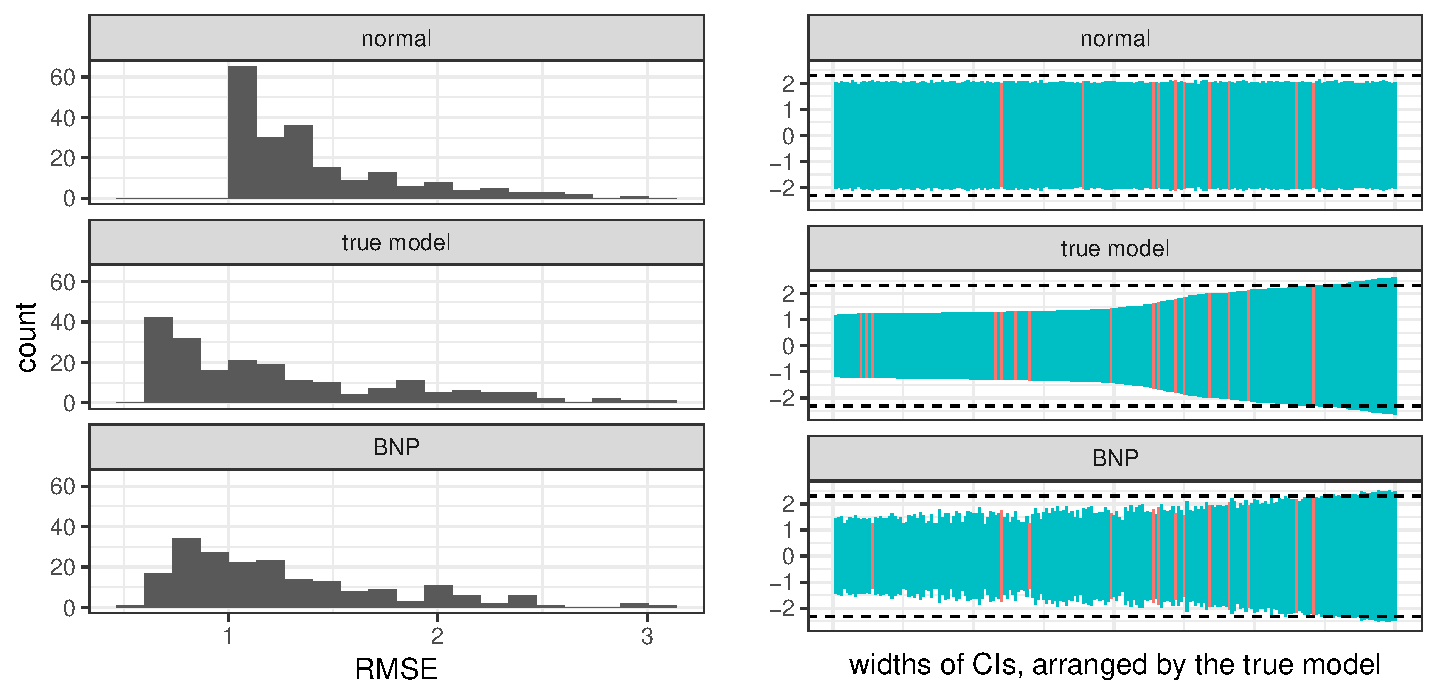
\includegraphics[width=.9\textwidth]{toy_ex/precision}
\begin{minipage}{.7\textwidth}\small%
\caption{Left: Histograms of the mean squared error based on posteriors for these models. Right: The widths of the 95\% posterior credible intervals for $\mu_g$ under the three hierarchical models, arranged by the width for the true model. Intervals which failed to cover the true value are colored red. The dashed lines correspond approximately to credible intervals with independent uniform priors on $\mu_g$.}
\end{minipage}
\label{precision}
\end{figure}


\subsection{BNP model for RNA-seq data}


\label{sec:model}
Let $y_{gn}$ represent the normalized log-cpm for gene $g$, sample $n$. Let $x_{n}^\top$ be the row of the design matrix $X$ corresponding to sample $n$. We will use the upper case letters $G$ and $N$, to denote the number of genes and samples, respectively. Also let $w_{gn}$ be the precision weight for $y_{gn}$. For the observed data, we assume the normal model
\begin{equation}
y_{gn} \sim \op{N} \left( x_{n}^\top \beta_g, \frac{\sigma^2_g}{w_{gn}} \right).
\end{equation}
Next, we propose to model jointly

\begin{equation}
\left(\beta_g^\top,\sigma^2_g\right) \ind \mathcal{P},
\end{equation}
where we specify a Dirichlet process on $\mathcal{P}$, i.e.,

\begin{equation}
\mathcal{P} \sim \op{DP}(\alpha \mbox{Q}).
\end{equation}

\iftoggle{thesis}{
The use of this prior, due to \citet{ferguson}, is a distribution over probability distributions, such that for any finite disjoint partition $\{A_i\}_{i>=1}^n$ on $\mathbb{R}^p$, $\mathcal{P}$ is a random measure such that the joint distribution $\left(\mathcal{P}(A_1),\ldots,\mathcal{P}(A_n)\right) \sim \op{Dir}\left(\alpha Q(A_1),\ldots,\alpha Q(A_n)\right).$ The Dirichlet process has two parameters: $Q$, the base measure, represents a prior guess at the distribution. $\alpha$, the concentration parameter expresses the degree to which $\mathcal{P}$ will agree with $Q$ on any set $A$. This follows from the definition given above and known properties of the Dirichlet distribution, i.e., $\op{E}\left(\mathcal{P}(A)\right)=Q(A)$, and $\op{V}\left(\mathcal{P}(A)\right)=\frac{Q(A)(1 - Q(A)}{\alpha + 1}$, showing that $\mathcal{P}(A) \stackrel{p}{\rightarrow} Q(A)$ as $\alpha \rightarrow \infty$ for any set $A$. 
}{}
By modeling $\mathcal{P}$ with a Dirichlet process one can be noninformative about the overall shape of $\mathcal{P}$, allowing for irregular shapes, multimodality, and so forth. An argument can be made that by incorporating our uncertainty about these features of the distribution is required for coherent interpretation of the posterior distribution \citep{walker2010bayesian}. For more information about the properties of the DP, see \cite{ferguson}.

As shown by \citet{sethuraman}, it follows from the definition of the Dirichlet process that $\mathcal{P}$ is almost surely discrete and realizations of $\mathcal{P}$ can be produced by the following stick-breaking construction:

Let 
\begin{equation}
\mathcal{P} =\sum_{k=1}^\infty \pi_k \delta_{\left(\tilde{\beta}_k^\top ,\tilde{\sigma}^2_k\right)}.
\end{equation}
Here $\delta_{(.)}$ is the Dirac delta function. Note that although almost sure discreteness is a property applicable to ``draws'' from a DP, the posterior for $\mathcal{P}$ is in fact a mixture of DP \citep{antoniak}. An implication of discretness can be thought of as a ``bet on sparsity"; that there are actually a finite (but unspecified) number of unique values that $(\beta_g^\top,\sigma^2_g)$ can take.  
 The ``atoms" distributed according to $Q$, specified by the product measure

\begin{equation}
\tilde{\beta}_k \sim \op{N}(m_\beta, C_\beta),\quad \tilde{\sigma}^2_k \sim \op{IG}(a_{\sigma^2}, b_{\sigma^2}).
\end{equation}

``$\op{IG}(a,b)$" refers to the inverse gamma distribution which we parameterize by shape and scale parameters, $a$ and $b$ with density given by
\begin{equation*}
p(x|a,b) = \frac{b^a}{\Gamma(a)}x^{a+1}e^{-b/x}.
\end{equation*}


The mixture weights, $\pi_k$,  follow a stick-breaking process \cite{sethuraman}. Using the reparameterization,

\begin{equation}
\nu_k = \frac{\pi_k}{1 - \sum_{l=1}^{k-1} \pi_l},
\end{equation}

$\nu_k$ representing a proportion of the total probability remaining after $k-1$ breaks. For the stick-breaking construction of the DP, the $\nu_k$ are modeled by:
\begin{equation}
\nu_k \ind \op{Beta}(1, \alpha).
\end{equation}

This assumption induces a stochastically decreasing ordering of the weights. Additionally, note that $\sum_{k=1}^K \pi_k \stackrel{p}{\rightarrow} 1$ as $K\rightarrow \infty$.

\subsection{Priors}
The base measure, $Q$, represents a prior guess at $\mathcal{P}$. The use of diffuse base measures is not recommended as it can result too few practically significant weights, $\pi_k$ \citep[p.554]{gelman-book}. For purposes of comparability, we set $Q$ by matching the quantiles of the empirical distribution of the independently obtained estimates of $\beta_g$, $\sigma_g^2$. The prior distribution for $\alpha$ was chosen by considering the implied expected number of clusters. Although we it is difficult to guess the number of clusters \textit{a priori}, we believe that most genes will have a pattern of expression that is similar to some other gene, so that after grouping the genes into clusters, the number of clusters should be much smaller than the number of genes. Also, due to computational constraints, we cannot deal with more than about 6000 clusters. We select the prior $\alpha \sim \op{Ga}(3,3/G^{0.5})$, which implies the expected number of clusters is likely between $G^{0.5}$ and $G^{0.75}$.
%For $\beta_gl$; $l=2,3,4,5$, these were obtained using the \texttt{estimateBetaPriorVar} from the \texttt{DESeq2} package using the ``quantile" method. For $\beta_g1$ and $\sigma^2_g$, a similar m

\section{Simulation study 1}
Since the proposed BNP method uses voom weights, we did a simulation study to compare the our method to the voom-limma method for RNA-seq data. The voom-limma method fits a linear model to the data under the same transformation conditional on the same voom quality weights, but proceeds by fitting each gene independently. Thus, a comparison of the estimates obtained under BNP model to the voom-limma estimates will show the result of borrowing information across genes via the Dirichlet process prior on $\mathcal{P}$.

\paragraph{Construction of simulated data:}
\begin{enumerate}
\item Select random draw of $\mathcal{P}$, $\mathcal{P}^{(s)}$, obtained from the posterior distribution given the entire Paschold data set

\item Sample $(\beta_g,\sigma^2_g)$ independently from $\mathcal{P}^{(s)}$, $g=1,\ldots,10000$ 

\item Sample $y_{g} \sim N(X\beta_g,\sigma^2_g I)$
\end{enumerate}
Produce 6-10 such data sets\\

A common goal of gene expression profiling is to produce a ranked list of 'called' genes for which a particular hypothesis is most likely to be true. The authors of \texttt{limma} provide multiple methods for calling genes. One method, called a ``TREAT", tests whether the log-fold-change due to a model term is larger than a specified threshold in absolute value, i.e. it allows users to ranking genes based on the evidence of the hypothesis, $H_{gl}:|\beta_{gl}|>t$. The test uses a moderated t-test that involves an shrunken estimates of$\sigma^2_g$. We can compare the ranking given by \texttt{limma} to ones based on posterior probabilites that $H_{gl}$ is true. The top panel of Figure \ref{roc-ss1} shows a typical receiver operator characteristic curve among the ten we observed. The bottom panel shows the area under the ROC curve (AUC) up to a FPR of 0.1. For both plots we show results for each component of $\beta$ (excluding the intercept) and a range of thresholds. In our simulations the BNP method tended to outperform \texttt{limma} on average. Note that while \texttt{limma} can perform tests with a threshold of zero, there is no comparable result for the BNP model, since this hypothesis has probability zero. The exception seems to be for the parental half-difference. For that particular set of tests, both \texttt{limma} and BNP appear to have similar accuracy.
%The comparative advantage seems to depend on the threshold: When $t=0$, there is little difference in the ROCs for testing $H_{g3}$, but as the threshold was increased to a log-fold change of 0.2, BNP outperformed \texttt{limma} by a wide margin.
% This suggests that our method, by ``learning" the underlying distribution of $\beta$, increases the ability to detect effects of practical significance.

\begin{figure}[h!]
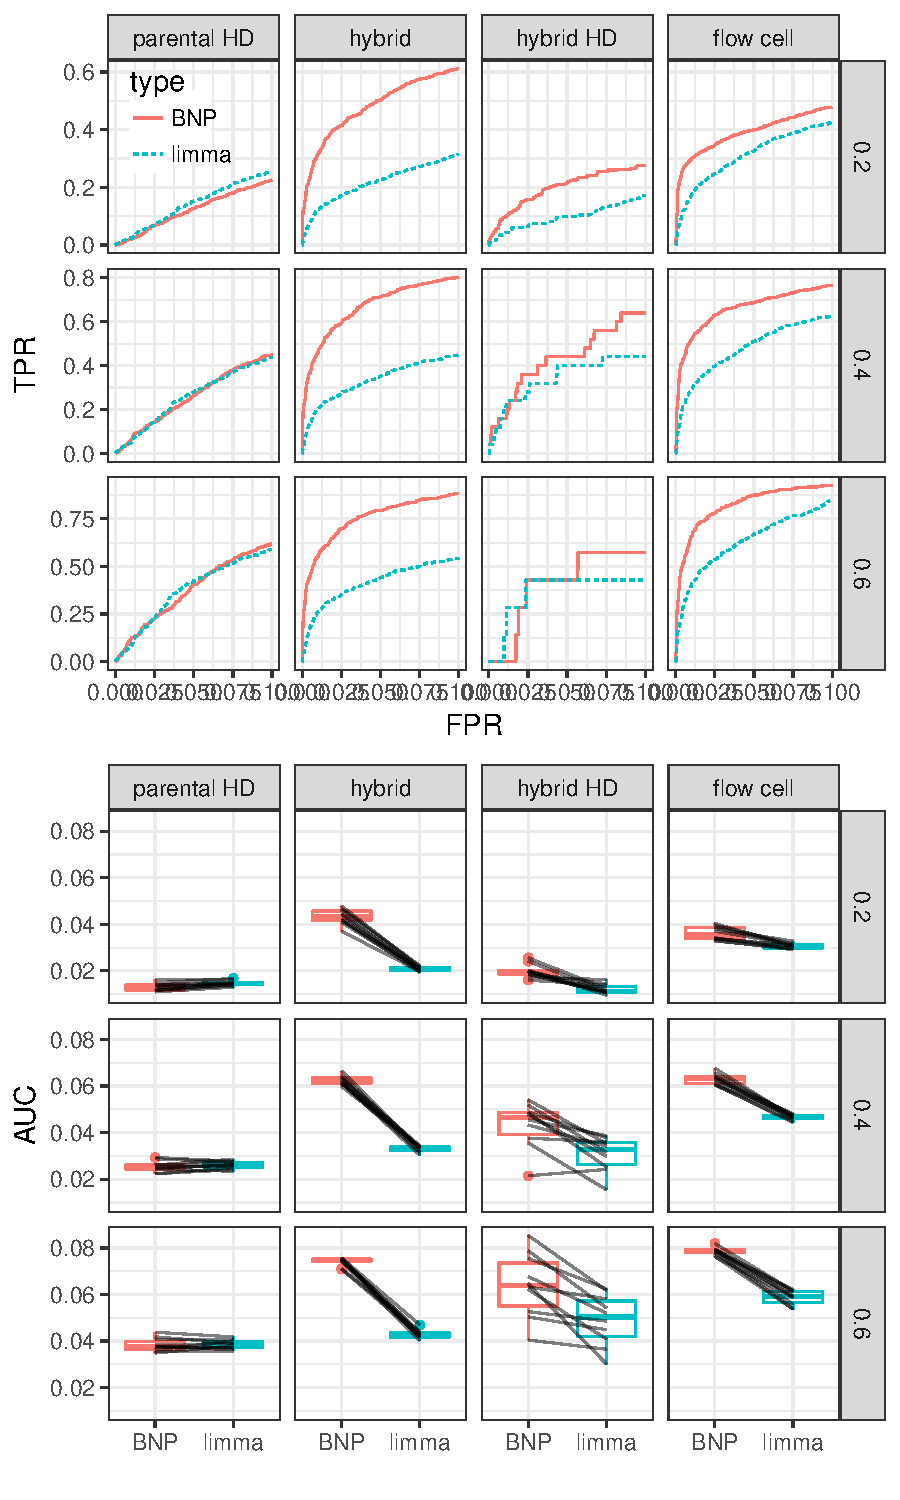
\includegraphics[width=.8\textwidth]{ss1-roc-auc}
\label{roc-ss1}
\end{figure}

We also compared the accuracy of point estimate under the two models. Here we expect BNP to do much better than \texttt{limma}. This is because \texttt{limma} produces point estimate for $\beta_g$ without any pooling of information, whereas the BNP provides shrinkage toward the mass of the underlying distribution of the $\beta_g$s. Figure \ref{mspe-ss1} shows that this is indeed the case; the mean squared prediction errors averaging across genes are uniformly smaller by approximately half relative to the same for \texttt{limma}.

\begin{figure}[h!]
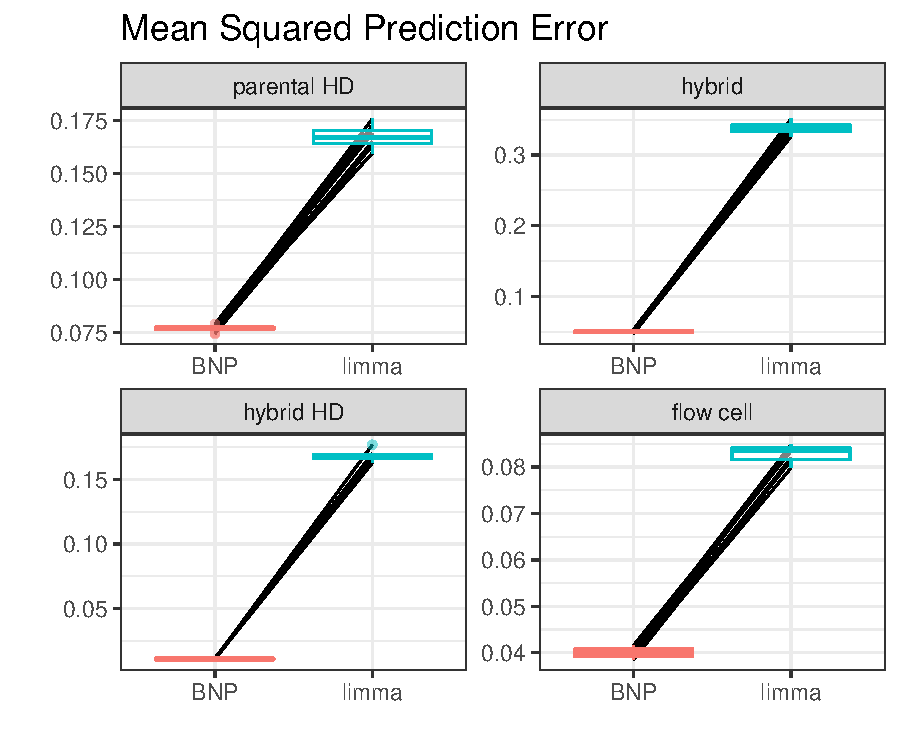
\includegraphics[width=.6\textwidth]{ss1-mspe}
\label{mspe-ss1}
\end{figure}

\section{Simulation study 2}
Much of the recent methods proposed for the analysis of RNA-seq data are based on an assumption that repeated sequencing of the same sample would produce Poisson distributed counts. For example, \cite{mccarthy} motivates the negative binomial model by showing that it has the right mean-variance relationship given the the above assumption and an assumption that the coefficient of variation is for constant within a gene. The favored approach is a negative binomial generalized linear model with log link function.

To compare estimation and accuracy of gene selection with existing methods designed for RNA-seq count data, we simulated count data by fitting the Paschold data with \texttt{voom/limma} and sampling a random subset of 10,000 genes without replacement. We then simulated normal data, conditioning on the estimates of $\beta_g$, $\sigma^2_g$, as well as the estimated precision weights. These simulated log-cpm values were then converted to log-counts, centering by $\log_2(\bar{R}_\cdot)-\log_2(10^6)$, where $\bar{R}_\cdot$ is the geometric mean of the estimated effective library sizes. Finally, these log-counts ($y_{gn}$) were exponentiated and rounded to obtain the simulated counts, $\tilde{y}_{gn}$. For each simulated data set, we analyzed the data using our BNP method and also with two popular count-based methods, DESeq2 and edgeR. For purposes of comparison, we considered accuracy of point estimation via mean squared prediction error and accuracy in identifying interesting genes using ROC curve.
% \begin{minipage}{.8\textwidth}
\begin{enumerate}
\item Sample 10,000 indices, $g$, from $\{1,2,\ldots,36,000\}$ without replacement.
\item Set $\beta_g:= \hat{\beta}_{voom,~g},\; \sigma^2_g:= \hat{\sigma}^2_{voom,~g}$
\item Sample $y_{gn} \sim \op{N}(x{gn}^\top\beta_g, \sigma^2_g/w_{gn})$
\item Set $\tilde{y}_{gn} = \op{Round} \left\{ 2^{y_{gn} + \log_2(10^6) - \log_2(\bar{R}_{\cdot})} \right\}$
\end{enumerate}
% \end{minipage}
% Mean squared prediction error
For each simulation we computed the mean squared prediction error (MSPE) corresponding to each element of $\beta_g$, $\frac{1}{G}\sum_{g=1}^G (\hat{\beta}_g-\beta_g)^2$ for both methods. The results, shown in Figure \ref{ss2-mspe}, show that estimation with BNP is more accurate with respect to MSPE than DESeq2.

\begin{figure}[h!]
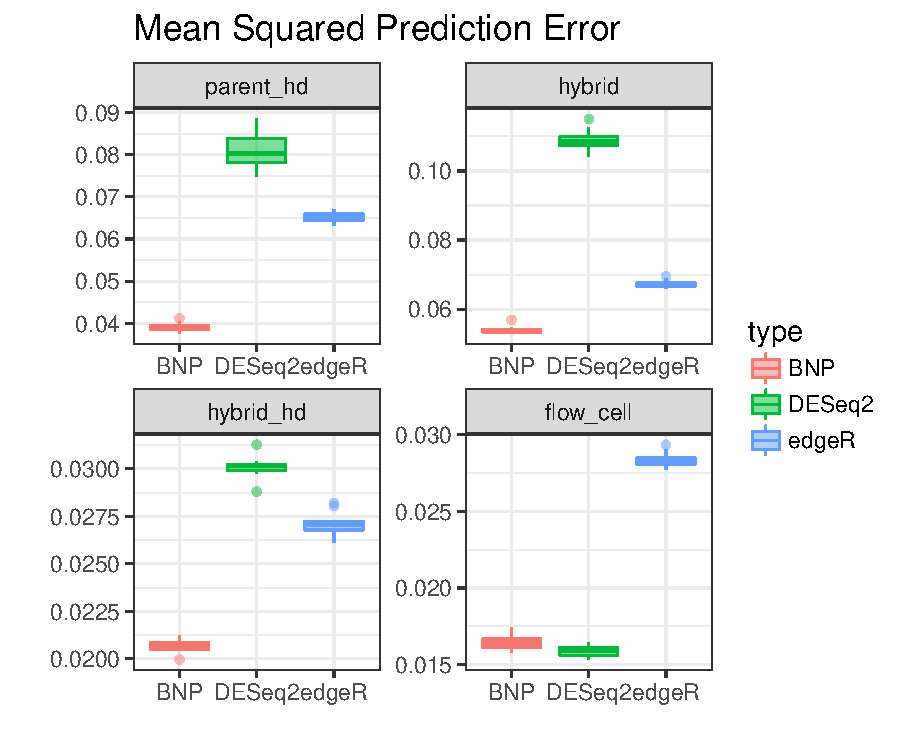
\includegraphics[width=.8\textwidth]{ss2-mspe}
\begin{minipage}{.8\textwidth}
\caption{\small Comparing the accuracy of estimation for BNP and DESeq2. Results show the average squared prediction error for 10 simulated data sets, grouped by function.}
\end{minipage}
\label{ss2-mspe}
\end{figure}
% Ranking accuracy (ROCs)

\begin{figure}[h!]
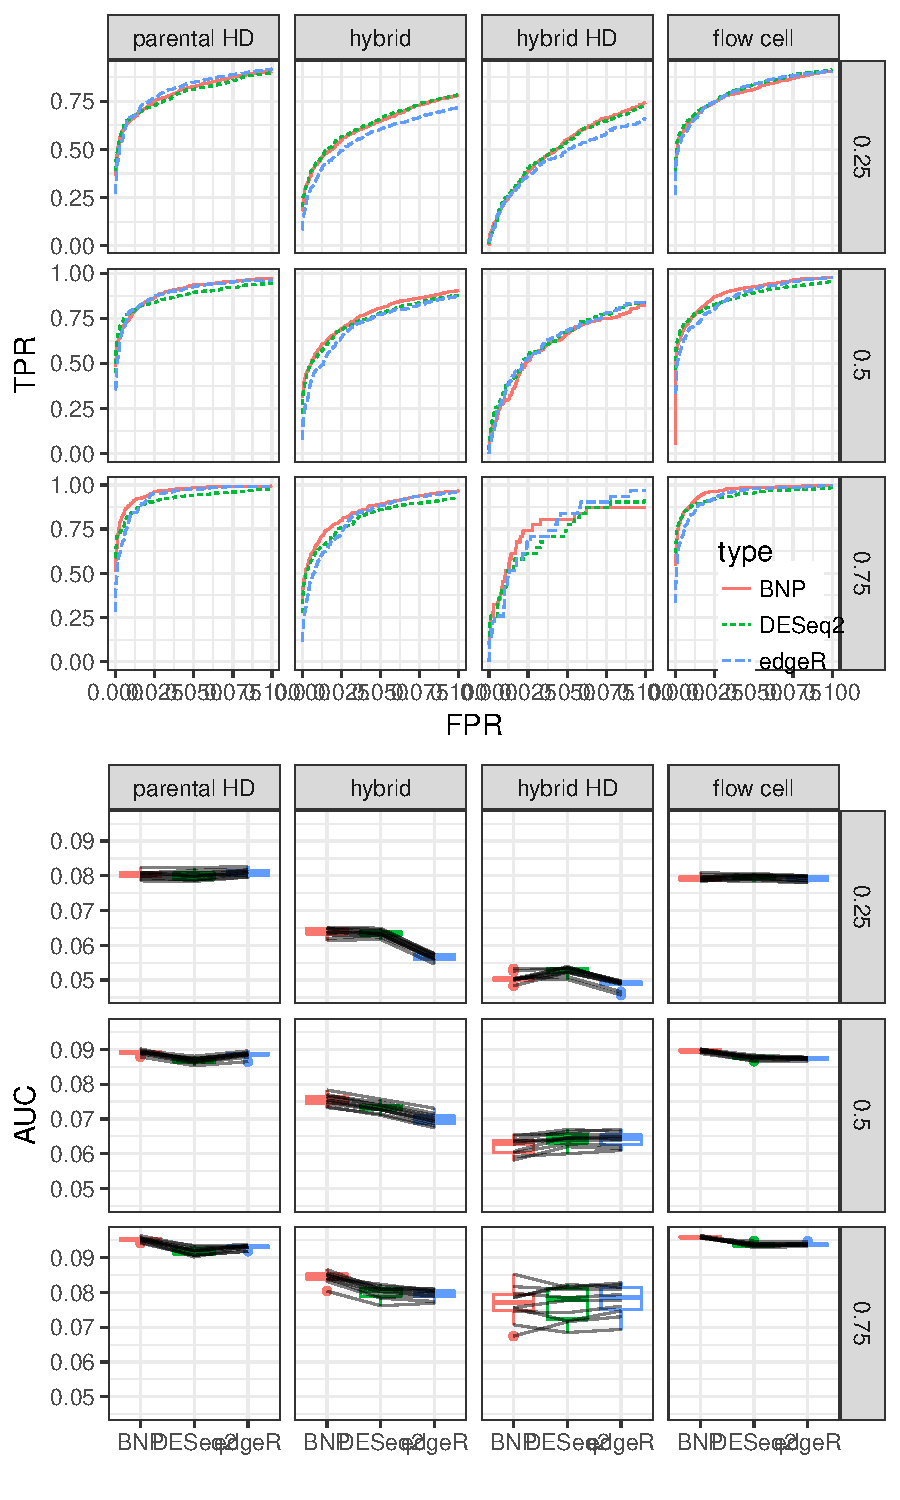
\includegraphics[width=.9\textwidth]{ss2-roc-auc}
\caption{\small ROCS.}
\label{ss2-roc}
\end{figure}

Simulation of counts:
To generate the simulated count data, we follow steps 1 and 2 of simulation study 1, and modify step 3: here, we bootstrap sample $W_{g,rep}$ from $W_g$ and simulate the pseudo-counts by
$$y^*_{g,rep} \sim N(X\beta_g,\sigma^2_gW_{g,rep}^{-1}).$$
Finally, we round $y^*_{g,rep}$ to obtain $y^*_{g,rep}$.




Generally: Generate count data, truth estimated from model, and compare voom pipelines.

Outputs: ROC curves, difference histograms

\section{Analysis of Paschold data}
To fit the Paschold data, we ran 4 chains, each for 40,000 iterations after 30,000 iterations of warmup. The samples were thinned by a factor of 40, for a total of 4,000 thinned post-warmup draws for each gene-specific parameter and $\alpha$. 




